% --
% theory

\section{Theory}\label{sec:nn_theory}
The most basic element in neural networks is denoted as node, an abstract element that defines input and output connections from and to other nodes within a network.
The edges of the connections from and to a node represents a multiplication with a scalar value, denoted as \emph{weight}.
Each node usually incorporates an additive term, denoted as \emph{bias term}.
All weights and bias terms are forming the parameters of a network and can be trained through backpropagation.
The output of a node is a scalar computed from all inputs and mapped with a non-linear function denoted as \emph{activation function}.
A neural network can consist of thousand of nodes in each possible constellation of connections.
The structure of a neural network is defined by its layers where a layer is a set of nodes with specific connection properties that receives input connections from the previous layer and outputs connections to the next layer.
For example, a neural network may consist of one convolutional layer followed by three fully-connected layers.
The last layer of a neural network usually represents the class labels regarding classification tasks.
A loss function computes the difference between the predicted and the actual class label during training and is essential for the backpropagation algorithm that updates each parameter in the network through the gradients of the obtained error.


% --
% activation functions

\subsection{Activation Functions}\label{sec:nn_theory_acti}
Activation functions for neural networks are usually present in each node and define non-linear functions that map the sum of the weighted input values from nodes in a previous layer to a single output value $z \in \R$ as follows:
\begin{equation}\label{eq:nn_theory_acti}
  z = h(\bm{w}^T \bm{x})
\end{equation}
where $h$ is the activation function, $\bm{w} \in \R^n$ is a weight vector and $\bm{x} \in \R^n$ an input vector representing the connections from a total number of $n$ nodes in the previous layer.
The output of each node in a current layer further connects to other nodes in the next layer, hence builds up the neural network.
The constraint of an activation function is that an easy computable derivative must exist.
This allows the backpropagation of gradients from the activation function.

The most famous activation function nowadays, is the Rectified Linear Unit (ReLU) \cite{Zeiler2013_relu} function:
\begin{equation}\label{eq:nn_theory_relu}
  h(a) = \max{(0, a)}
\end{equation}
with $a \in \R$ as input scalar.
The great advantage of the ReLU function is that its sub-gradients are very easy and fast computable.
Furthermore, two other well known activation functions used, for example, in the Wavenet, are the sigmoid function:
\begin{equation}\label{eq:nn_theory_sigmoid}
  h(a) = \frac{1}{1 + \exp{-a}}
\end{equation}
and the tanh function:
\begin{equation}\label{eq:nn_theory_tanh}
  h(a) = \frac{\exp{a} - \exp{-a}}{\exp{a} + \exp{-a}}
\end{equation}
where both squeeze the input between a range of either $[0, 1]$ for the sigmoid and $[-1, 1]$ for the tanh activation function.
\rfig{nn_theory_activation} illustrates the mentioned activation functions.
\begin{figure}[!ht]
  \centering
    \subfigure[ReLU]{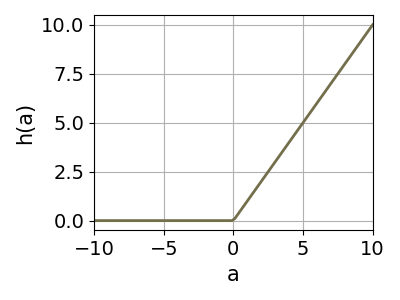
\includegraphics[width=0.3\textwidth]{./4_nn/figs/nn_theory_activation_relu.png}}
    \quad
    \subfigure[sigmoid]{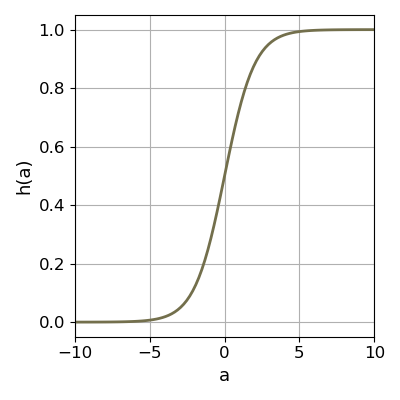
\includegraphics[width=0.3\textwidth]{./4_nn/figs/nn_theory_activation_sigmoid.png}}
    \quad
    \subfigure[tanh]{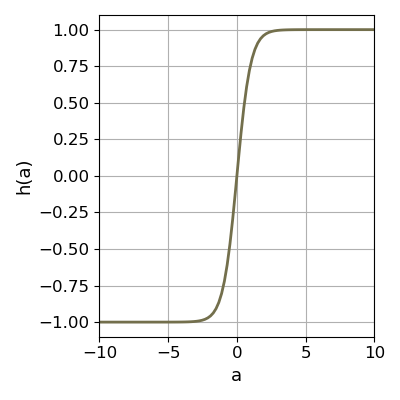
\includegraphics[width=0.3\textwidth]{./4_nn/figs/nn_theory_activation_tanh.png}}
  \caption{Different activation functions for neural networks.}
  \label{fig:nn_theory_activation}
\end{figure}
\FloatBarrier
\noindent


% --
% fully-connected

\subsection{Fully Connected Layer}
A fully-connected (FC) layer is one of the simplest and most commonly used layer types in neural network architectures.
Each node from a previous layer is forwardly connected to all nodes in a current FC layer.
A simple FC layer containing 3 nodes, is illustrated in \rfig{nn_theory_fc}.
% fc
\begin{figure}[!ht]
  \centering
    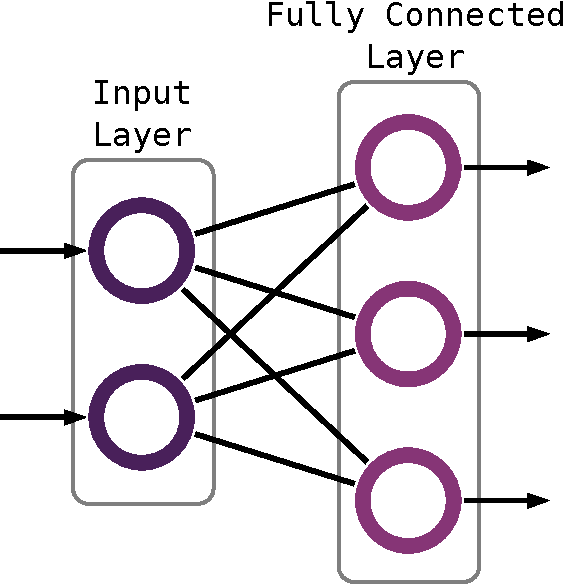
\includegraphics[width=0.30\textwidth]{./4_nn/figs/nn_theory_fc.pdf}
  \caption{Basic fully-connected layer with 3 nodes receiving connections from 2 input nodes and outputting connections to 2 output nodes.}
  \label{fig:nn_theory_fc}
\end{figure}
\FloatBarrier
\noindent
Mathematically one node $i$ performs the following calculation:
\begin{equation}
  z_i = h(\bm{w_i}^T \bm{x} + b_i)
\end{equation}
with the same notations as described in \req{nn_theory_acti} and an additional bias term $b_i \in \R$.
For all nodes in a current layer this equation of a single node can be summarized to a weight matrix $W \in \R^{m \times n}$ with $m$ as total amount of nodes in the current layer and a total number of $n$ nodes from the previous layer so that an FC layer can be defined as:
\begin{equation}
  \bm{z} = h(W \bm{x} + \bm{b})
\end{equation}
where $\bm{b} \in \R^m$ are the bias terms and $\bm{z} \in \R^m$ the outputs of all nodes in the current layer $m$.
With the matrix representation it is easy to obtain the number of training parameters and amount of operations needed for a FC layer.
The amount of parameters are clearly $m \cdot n$ for $W$ and $m$ for $\bm{b}$, so in total this results in $m \cdot n + m$ parameters.
The amount of operations are the matrix vector multiplication with approximated amounts of multiplication and additions, plus the additive bias terms.
Disregarding the activation function leads to an amount of calculations of approximately:
\begin{equation} 
  \mathcal{T}(W \bm{x} + \bm{b}) = 2 (m \cdot n) + m
\end{equation}
which would give, for example, with $n = 128$ and $m = 64$ roughly $\mathcal{T}(W \bm{x} + \bm{b}) = \SI{16.4}{\kilo\ops}$.


% --
% cnn

\subsection{Convolutional Layers}\label{sec:nn_theory_cnn}
Convolutional layers are the fundamental building block of every CNN, as already discussed in \rsec{prev_nn_cnn}.
Convolutional filters are applied on small areas of the input data to retrieve spatial information, where the input data may consist of multiple channels or input maps.
Those convolutional filters are also denoted as kernels $k$.
In the case the kernels operate on 2 dimensional input maps, they can be seen as 2 dimensional maps as well with kernel width $d_{k_w}$ and height $d_{k_h}$ typically smaller than the input maps.
The \emph{stride} of a kernel, denoted as $s$, specifies the number of shifts a kernel moves on a specific axis over an input map to perform the next convolution operation.
There are limited amounts of possible kernel strides over an input map in any specific axis, which determines the dimension of the output map on that axis.
The length $d_{o_z}$ of an output map of axis $z$ computes from an input map of length $d_{x_z}$ with a kernel striding along axis $z$ with $s_z$ and kernel size for that axis $d_{k_z}$ as follows:
\begin{equation}\label{eq:nn_theory_cnn_dim}
  d_{o_z} = \floor*{\frac{d_{x_z} + p_z - d_{k_z}}{s_z} + 1}
\end{equation}
where $p_z$ is an additional \emph{padding} term on the $z$ axis, which appends a specified amount of values to the input image on both sides of the selected axis.
Usually these appended values are zeros, such as applied in \emph{zero-padding}.
To provide an example of \req{nn_theory_cnn_dim}, consider the convolution of a $16 \times 16$ image by a $5 \times 5$ kernel with stride $1$ in each direction and without any padding terms, will result in an output image of dimensions $12 \times 12$.

A convolutional layer is therefore defined by the amount of input maps and resulting output channels (feature maps), the kernel size, the stride of the kernel, and some other specialties like padding and dilation.
Although it is not immediately clear from those parameters, how many convolutional filters are applied, and how the output feature maps are calculated in detail.
The number of convolutional filters $\#k$ is in most practical cases always:
\begin{equation}\label{eq:nn_theory_n_filters}
  \#k = i \cdot j
\end{equation}
where $i$ and $j$ is denoted as the amount of input and output channels respectively.
Each kernel produces a single feature map for each input channel, but the idea is to constraint the number of output maps $\#k$ to the defined output channels $j$.
This is usually done by summing up all feature maps obtained from all input channels $i$ convoluted with kernel $k_{i, j}$ for one specific output channel $j$ as follows:
\begin{equation}
  o_j = \sum_{i} k_{i, j} \ast x_i.
\end{equation}
where $o_j$ is the resulting j-th feature map or output channel, $x_i$ the i-th input channel, and $\ast$ represents the convolution operation.
\rfig{nn_theory_cnn_basics} provides a graphical example of the calculation of feature maps.
\begin{figure}[!ht]
  \centering
    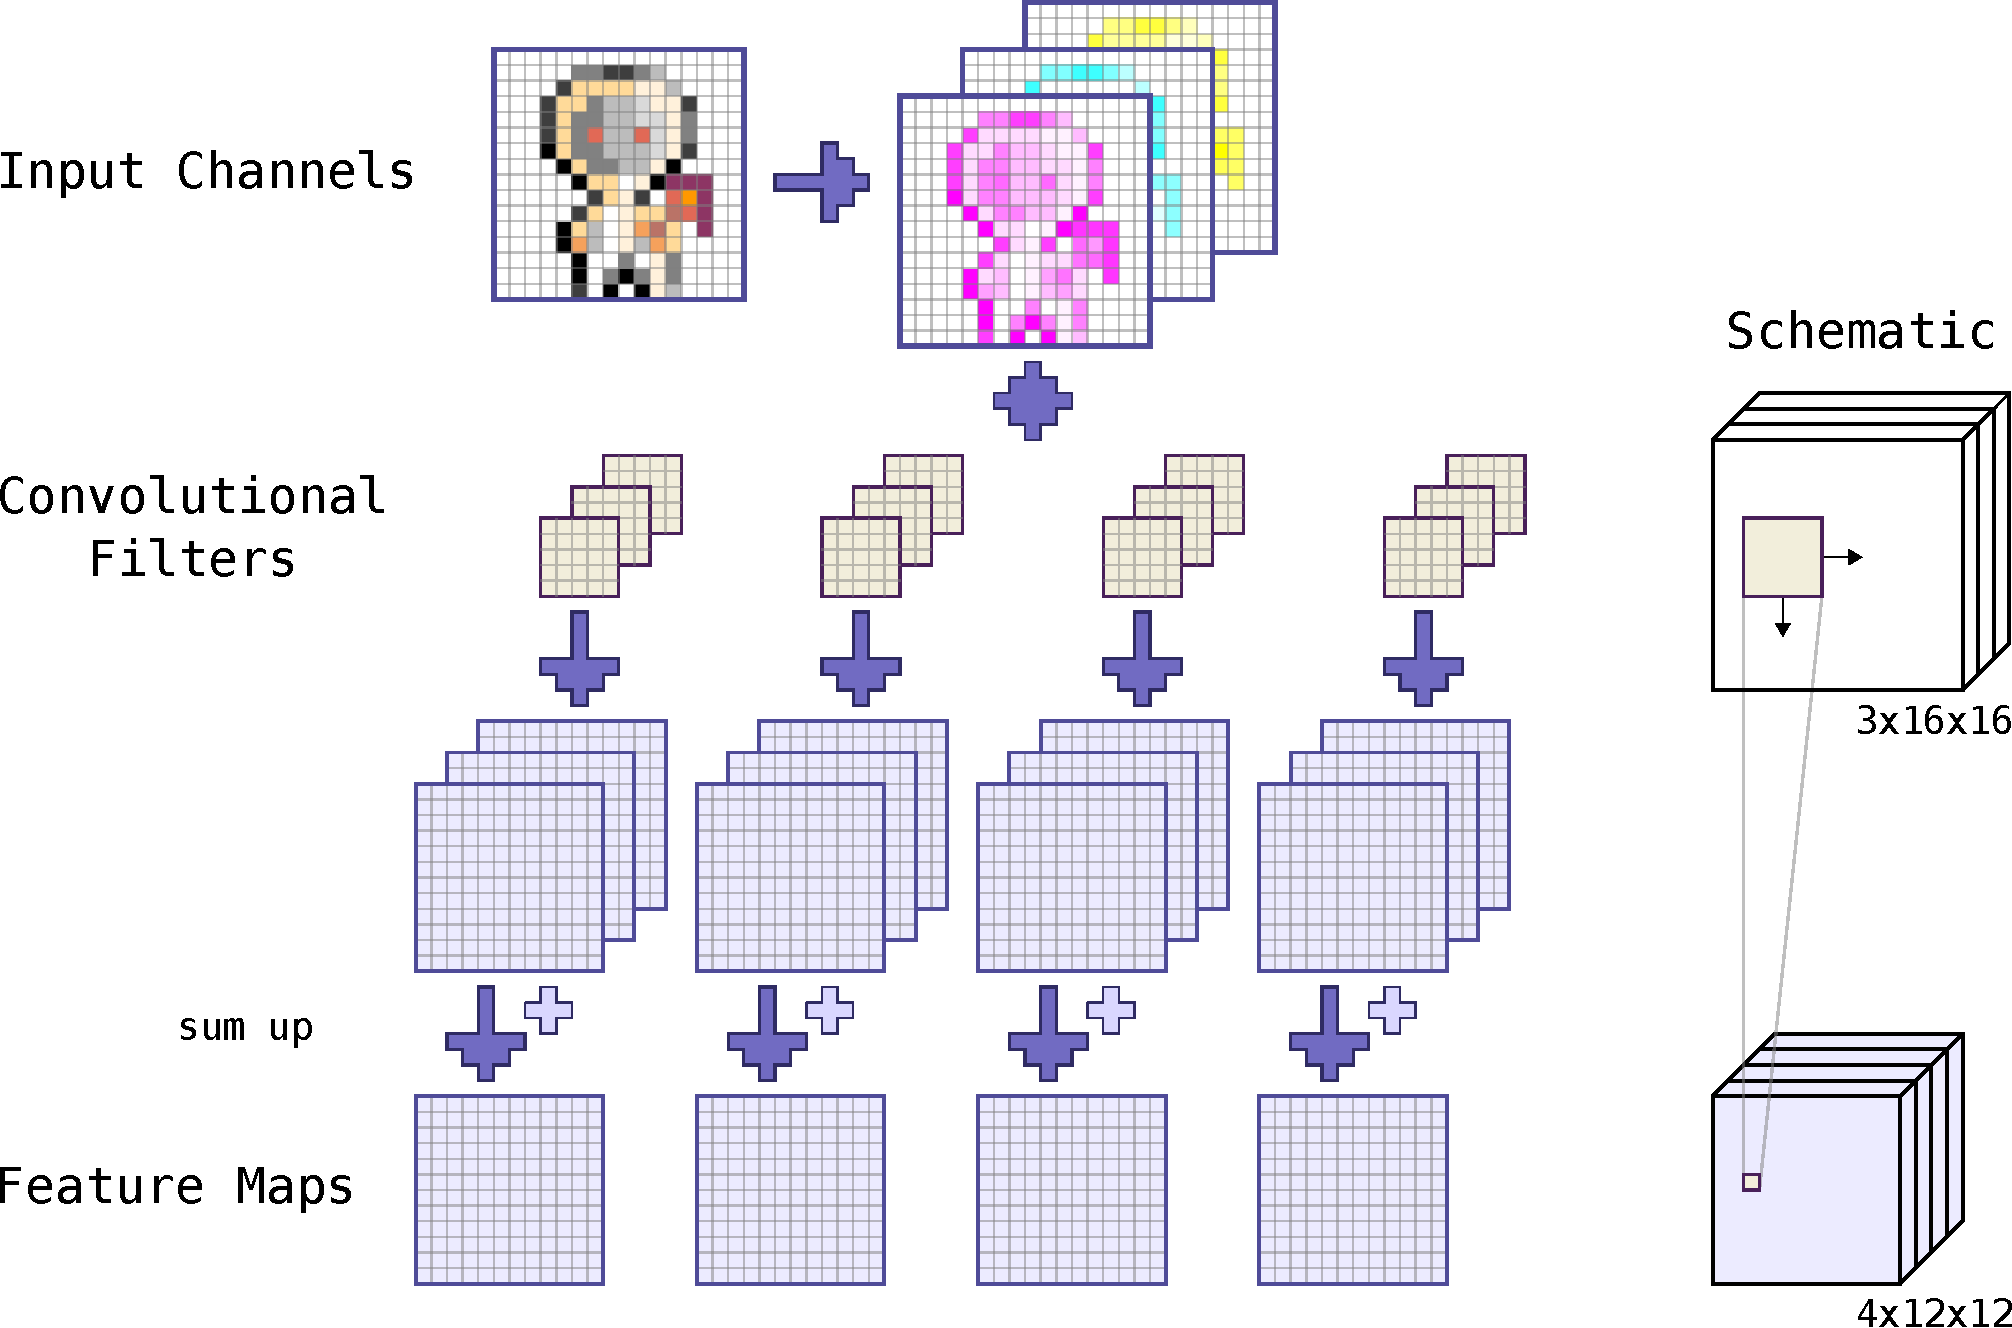
\includegraphics[width=0.75\textwidth]{./4_nn/figs/nn_theory_cnn_basics.pdf}
  \caption{Processing scheme of a convolutional layer composed of 3 input channels, 4 output channels, a kernel size of $5 \times 5$, and strides of $1$ in both dimensions. The input channel is represented by a $16 \times 16$ image decomposed in 3 color channels.}
  \label{fig:nn_theory_cnn_basics}
\end{figure}
\FloatBarrier
\noindent

The parameters of a convolutional layer consist of weights and bias terms in the convolutional filters.
However, the bias terms for each filter are optional.
By ignoring the bias terms, the amount of parameters are $\#k \cdot d_{k_w} \cdot d_{k_h}$ for a two dimensional convolutional layer, which makes $3 \cdot 4 \cdot 5 \cdot 5 = 300$ parameters for the example in \rfig{nn_theory_cnn_basics}.
The amount of operations of a convolutional layer is given by all convolution operations for each filter and the summation to $j$ output channels.
One convolution with a single two dimensional kernel $k$ and one input channel $x$ results in an approximate number of multiplication and addition operations:
\begin{equation}
  \mathcal{T}(k * x) = 2(d_{k_w} \cdot d_{k_h}) (d_{o_w} \cdot d_{o_h}).
\end{equation}
Further, the computation of all feature maps and their summation is given by:
\begin{equation}
  \mathcal{T}(o) = \#k \cdot \mathcal{T}(k * x) + \#k \cdot (d_{o_w} \cdot d_{o_h}).
\end{equation}
For the example in \rfig{nn_theory_cnn_basics}, this would result in $\mathcal{T}(k * x) = 2 (12 \cdot 12) (5 \cdot 5) = \SI{7.2}{\kilo\ops}$ and $\mathcal{T}(o) = 12 \cdot \SI{7.2}{\kilo\ops} + 12 \cdot (12 \cdot 12) = \SI{88.1}{\kilo\ops}$.


% --
% loss functions

\subsection{Loss Functions and Softmax}
Loss functions, also called cost functions, are used to determine the difference between the predicted label $\hat{y}_i$ for class $i$ compared to the actual or ground truth label $y$ of one specific training data example.
The predicted labels are usually presented by the output nodes in the last layer of a neural network.
Therefore, $\hat{\bm{y}} = [\hat{y_0}, \hat{y_1}, \dots, \hat{y_L}]^T$ has the dimension of the number of labels or classes $L$.
Often it is preferred that $\hat{\bm{y}} \in \R^L$ provides a probability distribution such that:
\begin{equation}
  \sum_{i=0}^L \hat{y}_i = 1
\end{equation}
which can be achieved with the softmax function:
\begin{equation}\label{eq:nn_theory_softmax}
  \hat{y}_i = \frac{\exp{x_i}}{\sum_{j=0}^{L}\exp{x_j}}
\end{equation}
in the last layer where $x$ presents here the output of any specific node.

There are already plenty of different loss functions available for training neural networks, such as described in \cite{LeCun2006}. 
In this thesis however, only one kind of loss function is applied for all neural network architectures namely the \emph{cross-entropy loss}, which is in the case of two classes known as \emph{binary cross-entropy loss}.
The formulation of the cross-entropy loss is similarly expressed as provided in the documentation of its implementation in the \texttt{Pytorch} framework \cite{Pytorch}.
The binary cross-entropy is implemented as:
\begin{equation}\label{eq:nn_theory_binary_cross_entropy}
  l(x_i, y_i) = y_i \cdot \log x_i + (1 - y_i) \cdot \log (1 - x_i)
\end{equation}
with the training pair $(x_i, y_i)$, where $x_i \in \R^{N \times 1}$ is the feature input and $y_i \in \{0, 1\}^N$ the corresponding label.
During the training procedure a whole batch with a total number of $N$ examples is used for one update step.
However, the loss function should provide only a single output value, which can be achieved by calculating the mean value of all $l_i$ where $i = 0, \dots, N$ is the index of the examples in the actual batch.

The multi-class variant of the cross-entropy is defined by:
\begin{equation}
  l(x_i, y_i) = - x_i[y_i] + \log{\left( \sum_{j=0}^{L} \exp{x_i[j]} \right)}
\end{equation}
with dimensions of the training pair $x_i \in \R^{N \times L}$ and $y_i \in \{0, 1, \dots, L\}^N$, and a total number of $L$ classes.
Note that $x_i[.]$ is denoted as indexing of $x_i$ of its class dimension $L$. 


% --
% dropout

\subsection{Dropout}
Dropout \cite{Hinton2012} is a method to improve generalization and training of neural networks.
The idea is to set the output of randomly selected nodes within a layer for one training step to zero so that only the other nodes are updated.
This can be done by multiplying all outputs of a current layer with a vector containing a specified number of zeros and ones places at random positions within the vector.
The amount of zeros compared to ones can be sampled from a Bernoulli distribution by setting a probability value $p$.
For instance, $p=0.2$ means that there are \SI{20}{\percent} zeros and \SI{80}{\percent} ones randomly placed within the vector.


% --
% training

\subsection{Training of a Neural Network}
The training of a neural network is usually done by updating each parameter of the model with back-propagated gradients from the obtained loss at the output nodes.
The loss is calculated by a specific loss function comparing the predicted labels to the targets of the actual training samples.
To update the parameters of the network, an update rule, such as Stochastic Gradient Descend (SGD) or Adam \cite{Kingma2015} is applied.
Note that a single update step is usually not performed on the whole dataset, unless it is a very small dataset. 
In the normal case the update is performed on small chunks of the dataset called \emph{batch}.
One training iteration is therefore the update of parameters for a single batch.
The run over all batches of a dataset is defined as \emph{epoch}.
Note that the training of neural networks may take over thousands of epochs until convergence is reached.
The general training techniques for neural networks and further details are not described because of many existing books and papers, such as \cite{LeCun2006}, \cite{Goodfellow2016}, \cite{DeepLearning}, that are already presenting this topic very well. 
Moreover, it does not add any value to this thesis as the algorithms are well examined and run in the background of every neural network framework.
Hence, the interesting elements are only the neural network architecture design, the hyperparameters for training, and the used loss functions.


% --
% GANs

\subsection{Generative Adversarial Neural Networks Game}\label{sec:nn_theory_gan}
GANs \cite{Goodfellow2014}, as already mentioned in \rsec{prev_nn_adv} consist of two neural networks: a Generator (G) network for generating fake images and a Discriminator (D) network for discriminating between fake and real images.
The min-max game both networks are playing, is defined by:
\begin{equation}\label{eq:nn_theory_gan}
  \underset{G}{\min} \, \underset{D}{\max} \, V(D, G) = \E_{\bm{x} \sim p_{data}(\bm{x})}\left[ \log D(\bm{x}) \right] + 
    \E_{\bm{z} \sim p_{\bm{z}}(\bm{z})}\left[ \log (1 - D(G(\bm{z}))) \right]
\end{equation}
where $\bm{x} \in \mathcal{X}$ are samples from the training data $p_{data}$, $\bm{z} \in \mathcal{Z}$ is a latent variable sampled from $p_{\bm{z}}$, $D: \mathcal{X} \mapsto [0, 1]$ is the discriminator network and $G: \mathcal{Z} \mapsto \mathcal{X}$ the generator network.
The advise from the original paper is not to minimize G with $\log (1 - D(G(\bm{z})))$ but to maximize $\log D(G(\bm{z}))$ instead.